% Start writing your answer from here, if you want to use new packages/change something do it in main.tex
\begin{que}
	Download the image of Monalisa from here. Read the image using matplotlib (example). Write a
	piece of python code to shift the image along the X direction by tx pixels where tx is an integer
	ranging from -10 to +10 (so, in total you need to do this for 20 values). While doing so, assign
	a value of 0 to unoccupied pixels. For each shift, compute the correlation coefficient between the
	original image and its shifted version. Make a plot of correlation coefficients across the shift values.
	Also, generate a normalized histogram for the original image. You might need to refer to section
	3.3 from this book. You are not allowed to use any inbuilt function for generating the histogram.
	If you are using any other libraries, then please mention about them in the pdf.

	\hspace*{\fill} [8 marks]
\end{que}

\begin{tcolorbox}[breakable]
	\begin{sol}
		The image of Mona Lisa was read using the \texttt{matplotlib} library. The image was then shifted horizontally by \texttt{tx} pixels for each value of \texttt{tx} in the range of -10 to +10. The shifting operation was implemented manually, ensuring that unoccupied pixels were assigned a value of 0.

		A custom function \texttt{shiftimg} was created to handle the shifting process:
		\begin{itemize}
			\item If \texttt{tx > 0}, pixels were shifted rightwards by \texttt{tx} units.
			\item If \texttt{tx < 0}, pixels were shifted leftwards by \texttt{tx} units.
			\item If \texttt{tx = 0}, the function returned the original image.
		\end{itemize}

		For each shifted image, the correlation coefficient between the original and shifted image was calculated. This coefficient quantifies the linear relationship between the two images, with values ranging from -1 to 1, where 1 indicates a perfect positive correlation, -1 indicates a perfect negative correlation, and 0 indicates no correlation.
		A normalized histogram of the original image was generated by calculating the frequency of each pixel intensity and then normalizing the values. This was done manually without using any inbuilt histogram function.
		\newpage
		The correlation coefficients for the different shift values were plotted to observe the relationship between the magnitude of the shift and the correlation with the original image.

		\begin{figure}[H]
			\centering
			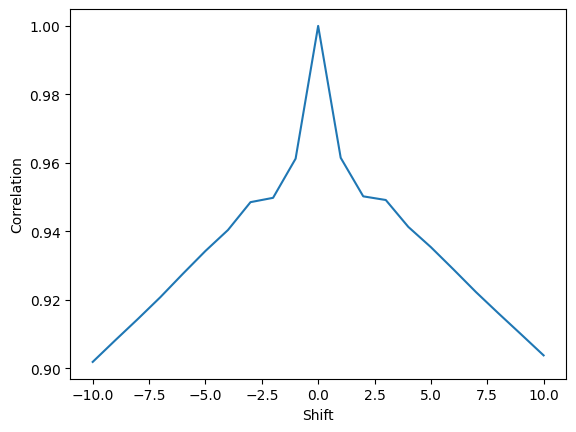
\includegraphics[width=0.8\textwidth]{correlation_plot.png}
			\caption{Correlation Coefficient vs Shift Values}
			\label{fig:corr_plot}
		\end{figure}


		As observed in Figure \ref{fig:corr_plot}, the correlation decreases as the shift increases in either direction. This is expected as the more the image is shifted, the less it resembles the original, resulting in lower correlation values.

		The normalized histogram of the original image was also plotted to visualize the distribution of pixel intensities.

		\begin{figure}[H]
			\centering
			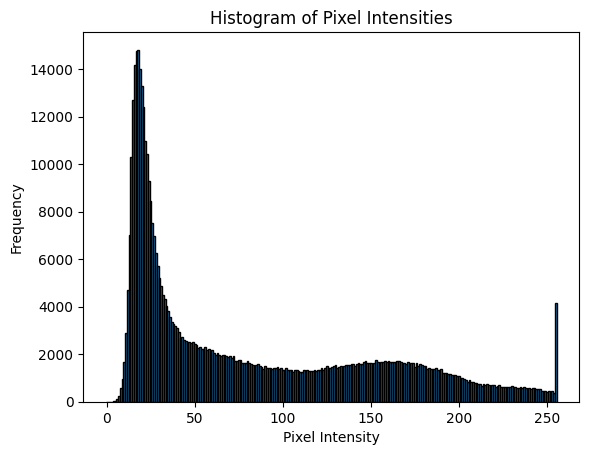
\includegraphics[width=0.5\textwidth]{red_pixel_intensity.png}
			\caption{Normalized Histogram of the Original Image}
			\label{fig:hist_plot}
		\end{figure}

		The histogram in Figure \ref{fig:hist_plot} shows the frequency of occurrence of each pixel intensity, normalized over the total number of pixels.




	\end{sol}
\end{tcolorbox}
